% sosoft-card.tex — Score for Social Software deck card
% Jeffrey Alan Scudder — "$roz" (KidLisp program as score)
% Card size: 2.75in × 4.75in (70mm × 120mm)
% Full-color KidLisp syntax highlighting (light mode palette)
%
% Build: cd sosoft && xelatex card.tex

\documentclass[12pt]{article}
\usepackage[
  paperwidth=2.75in,
  paperheight=4.75in,
  top=0.3in,
  bottom=0.3in,
  left=0.3in,
  right=0.3in,
]{geometry}
\usepackage{fontspec}
\usepackage{xcolor}
\usepackage{tikz}
\usepackage{listings}
\usepackage{setspace}
\usepackage{graphicx}

\pagestyle{empty}

% === FONTS ===
\newfontfamily\acbold{ywft-processing-bold}[
  Path=../system/public/type/webfonts/,
  Extension=.ttf
]
\newfontfamily\aclight{ywft-processing-light}[
  Path=../system/public/type/webfonts/,
  Extension=.ttf
]
\setmonofont{Nimbus Mono PS}

% === KidLisp light-mode palette ===
\definecolor{ink}{RGB}{0,0,0}
\definecolor{faint}{RGB}{140,140,140}
\definecolor{klfn}{HTML}{0099cc}
\definecolor{klform}{HTML}{cc00cc}
\definecolor{klnum}{HTML}{cc0066}
\definecolor{klident}{HTML}{cc6600}
\definecolor{klgreen}{HTML}{2e8b57}
\definecolor{klmath}{HTML}{00aa00}
\definecolor{klcmt}{HTML}{666666}
\definecolor{p0}{RGB}{255,100,100}
\definecolor{p1}{RGB}{255,180,100}
\definecolor{p4}{RGB}{100,200,255}
\definecolor{klred}{RGB}{255,0,0}
\definecolor{klblue}{RGB}{0,0,255}
\definecolor{klblack}{RGB}{0,0,0}
\definecolor{klcyan}{RGB}{0,200,200}
\definecolor{klyellow}{HTML}{cc9900}
\definecolor{klmagenta}{RGB}{200,0,200}
\definecolor{klwhite}{RGB}{180,180,180}
\definecolor{rb0}{HTML}{ff0000}
\definecolor{rb1}{HTML}{ff7f00}
\definecolor{rb2}{HTML}{ffff00}
\definecolor{rb3}{HTML}{00ff00}
\definecolor{rb4}{HTML}{0000ff}
\definecolor{rb5}{HTML}{4b0082}
\definecolor{rb6}{HTML}{9400d3}
% Inverse colors for shadows (255-r, 255-g, 255-b)
\definecolor{invfn}{RGB}{255,102,51}      % inverse of cyan 0099cc
\definecolor{invnum}{RGB}{51,255,153}     % inverse of pink cc0066
\definecolor{invident}{RGB}{51,153,255}   % inverse of orange cc6600
\definecolor{invgreen}{RGB}{209,116,168}  % inverse of 2e8b57
\definecolor{invred}{RGB}{0,255,255}      % inverse of red
\definecolor{invblue}{RGB}{255,255,0}     % inverse of blue
\definecolor{invblack}{RGB}{255,255,255}  % inverse of black
\definecolor{invcyan}{RGB}{255,55,55}     % inverse of 0,200,200
\definecolor{invyellow}{RGB}{51,102,255}  % inverse of cc9900
\definecolor{invmagenta}{RGB}{55,255,55}  % inverse of 200,0,200
\definecolor{invwhite}{RGB}{75,75,75}     % inverse of 180,180,180
\definecolor{invp0}{RGB}{0,155,155}       % inverse of paren red
\definecolor{invp1}{RGB}{0,75,155}        % inverse of paren orange

\lstdefinestyle{kidlisp-card}{
  basicstyle=\ttfamily\fontsize{6.5pt}{11.5pt}\selectfont\color{ink},
  breaklines=false,
  frame=none,
  xleftmargin=0pt,
  aboveskip=0pt,
  belowskip=0pt,
  columns=fixed,
  keepspaces=true,
  showstringspaces=false,
  escapechar=|,
}

% Shorthand macros
\newcommand{\fn}[1]{{\color{klfn}\textbf{#1}}}
\newcommand{\xf}[1]{{\color{klfn}#1}}
\newcommand{\nm}[1]{{\color{klnum}#1}}
\newcommand{\id}[1]{{\color{klident}#1}}
\newcommand{\cn}[2]{{\color{#1}#2}}
\newcommand{\pr}[2]{{\color{#1}#2}}

% Shadow macro — #1 is the inverse/opposite color, rendered at 50% behind text
\newcommand{\sh}[2]{%
  \setbox0=\hbox{#2}%
  \rlap{\raisebox{-0.4pt}{\hspace{0.4pt}{\color{#1!50}\copy0}}}%
  \box0%
}
% Per-character rainbow (inverse shadow: 255-r, 255-g, 255-b per char)
% rb0=ff0000→inv 00ffff, rb1=ff7f00→inv 0080ff, rb2=ffff00→inv 0000ff
% rb3=00ff00→inv ff00ff, rb4=0000ff→inv ffff00, rb5=4b0082→inv b4ff7d, rb6=9400d3→inv 6bff2c
\definecolor{irb0}{RGB}{0,255,255}
\definecolor{irb1}{RGB}{0,128,255}
\definecolor{irb2}{RGB}{0,0,255}
\definecolor{irb3}{RGB}{255,0,255}
\definecolor{irb4}{RGB}{255,255,0}
\definecolor{irb5}{RGB}{180,255,125}
\definecolor{irb6}{RGB}{107,255,44}
\newcommand{\rbow}{%
  \sh{irb0}{\color{rb0}r}%
  \sh{irb1}{\color{rb1}a}%
  \sh{irb2}{\color{rb2}i}%
  \sh{irb3}{\color{rb3}n}%
  \sh{irb4}{\color{rb4}b}%
  \sh{irb5}{\color{rb5}o}%
  \sh{irb6}{\color{rb6}w}%
}

\begin{document}

% === Full-bleed faded background ===
\begin{tikzpicture}[remember picture, overlay]
  \node[anchor=center, inner sep=0pt, opacity=0.35]
    at (current page.center)
    {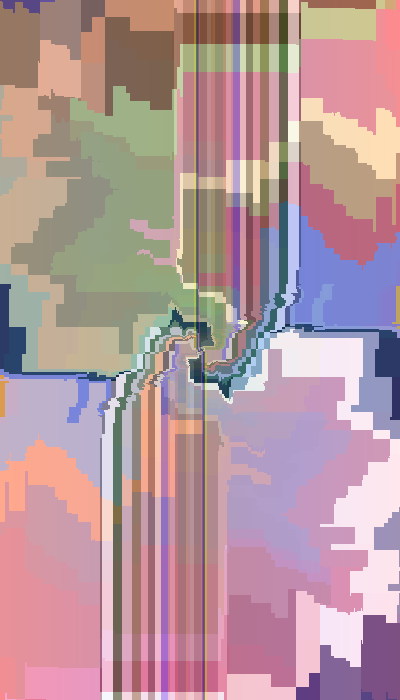
\includegraphics[width=2.8in, height=4.8in]{roz-bg.png}};
  % Safety margin guide (144px from edge at 652 DPI = 0.22in)
  \draw[red, line width=0.3pt, opacity=0.4]
    ([xshift=0.22in, yshift=-0.22in]current page.north west)
    rectangle
    ([xshift=-0.22in, yshift=0.22in]current page.south east);
\end{tikzpicture}

\vspace*{0.1in}

% === Small square $roz screenshot above the code ===
\begin{center}
  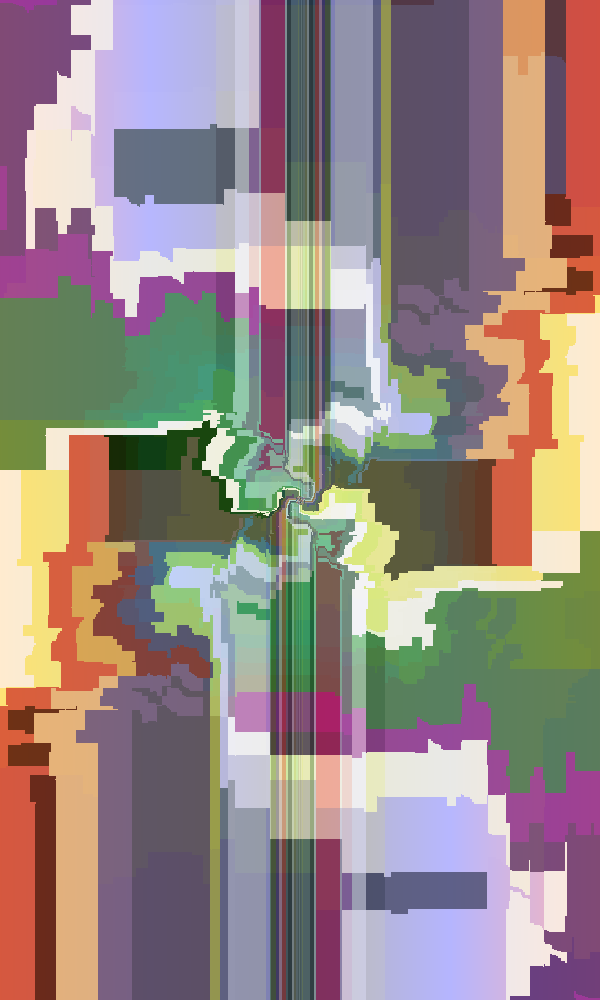
\includegraphics[width=1.9in, height=1.9in]{roz-screenshot.png}
\end{center}

\vspace{0.1in}

% === Source code with white backing (only behind code area) ===
\begin{tikzpicture}[remember picture, overlay]
  \fill[white, opacity=0.7, rounded corners=3pt]
    ([xshift=0.15in, yshift=-2.95in]current page.north west)
    rectangle
    ([xshift=-0.15in, yshift=0.1in]current page.south east);
\end{tikzpicture}
\begin{lstlisting}[style=kidlisp-card]
|\sh{invgreen}{\cn{klgreen}{fade}}|:|\sh{invred}{\cn{klred}{red}}|-|\sh{invblue}{\cn{klblue}{blue}}|-|\sh{invblack}{\cn{klblack}{black}}|-|\sh{invblue}{\cn{klblue}{blue}}|-|\sh{invred}{\cn{klred}{red}}|
|\sh{invfn}{\fn{ink}}| |\sh{invp0}{\pr{p0}{(}}||\sh{invfn}{\fn{?}}| |\rbow| |\sh{invwhite}{\cn{klwhite}{white}}| |\sh{invnum}{\nm{0}}||\sh{invp0}{\pr{p0}{)}}| |\sh{invp0}{\pr{p0}{(}}||\sh{invnum}{\nm{1s}}|... |\sh{invnum}{\nm{24}}| |\sh{invnum}{\nm{64}}||\sh{invp0}{\pr{p0}{)}}|
|\sh{invfn}{\fn{line}}| |\sh{invident}{\id{w}}|/|\sh{invnum}{\nm{2}}| |\sh{invnum}{\nm{0}}| |\sh{invident}{\id{w}}|/|\sh{invnum}{\nm{2}}| |\sh{invident}{\id{h}}|
|\sh{invp0}{\pr{p0}{(}}||\sh{invfn}{\xf{spin}}| |\sh{invp1}{\pr{p1}{(}}||\sh{invnum}{\nm{2s}}|... |\sh{invnum}{\nm{-1.125}}| |\sh{invnum}{\nm{1.125}}||\sh{invp1}{\pr{p1}{)}}||\sh{invp0}{\pr{p0}{)}}| |\sh{invp0}{\pr{p0}{(}}||\sh{invfn}{\xf{zoom}}| |\sh{invnum}{\nm{1.1}}||\sh{invp0}{\pr{p0}{)}}|
|\sh{invp0}{\pr{p0}{(}}||\sh{invnum}{\nm{0.5s}}| |\sh{invp1}{\pr{p1}{(}}||\sh{invfn}{\xf{contrast}}| |\sh{invnum}{\nm{1.05}}||\sh{invp1}{\pr{p1}{)}}||\sh{invp0}{\pr{p0}{)}}|
|\sh{invp0}{\pr{p0}{(}}||\sh{invfn}{\xf{scroll}}| |\sh{invp1}{\pr{p1}{(}}||\sh{invfn}{\fn{?}}| |\sh{invnum}{\nm{-0.1}}| |\sh{invnum}{\nm{0}}| |\sh{invnum}{\nm{0.1}}||\sh{invp1}{\pr{p1}{)}}| |\sh{invp1}{\pr{p1}{(}}||\sh{invfn}{\fn{?}}| |\sh{invnum}{\nm{-0.1}}| |\sh{invnum}{\nm{0}}| |\sh{invnum}{\nm{0.1}}||\sh{invp1}{\pr{p1}{)}}||\sh{invp0}{\pr{p0}{)}}|
|\sh{invfn}{\fn{ink}}| |\sh{invp0}{\pr{p0}{(}}||\sh{invfn}{\fn{?}}| |\sh{invcyan}{\cn{klcyan}{cyan}}| |\sh{invyellow}{\cn{klyellow}{yellow}}| |\sh{invmagenta}{\cn{klmagenta}{magenta}}||\sh{invp0}{\pr{p0}{)}}| |\sh{invnum}{\nm{8}}|
|\sh{invfn}{\fn{circle}}| |\sh{invident}{\id{w}}|/|\sh{invnum}{\nm{2}}| |\sh{invident}{\id{h}}|/|\sh{invnum}{\nm{2}}| |\sh{invp0}{\pr{p0}{(}}||\sh{invfn}{\fn{?}}| |\sh{invnum}{\nm{2}}| |\sh{invnum}{\nm{4}}| |\sh{invnum}{\nm{8}}||\sh{invp0}{\pr{p0}{)}}|
\end{lstlisting}

\vspace*{\fill}

% === QR code + label in bottom-right corner ===
\begin{tikzpicture}[remember picture, overlay]
  \node[anchor=south east, inner sep=0pt]
    at ([xshift=-0.3in, yshift=0.8in]current page.south east)
    {\colorbox{black}{%
      \rule[-1pt]{0pt}{6.5pt}%
      \kern-1pt{\ttfamily\fontsize{7.5pt}{7.5pt}\selectfont\color{white}\$roz}\kern-0.5pt%
    }};
  \node[anchor=south east, inner sep=1pt, fill=black!60]
    at ([xshift=-0.28in, yshift=0.28in]current page.south east)
    {\rule{0.48in}{0.48in}};
  \node[anchor=south east, inner sep=1pt, fill=white]
    at ([xshift=-0.3in, yshift=0.3in]current page.south east)
    {
\includegraphics[width=0.48in]{qr-roz.eps}};
\end{tikzpicture}

\end{document}
